% !TeX root = ../thesis_main.tex

% ---------------------------------------------------
% ----- Chapters of the template
% ----- for Bachelor-, Master thesis and class papers
% ---------------------------------------------------
%  Created by C. Müller-Birn on 2012-08-17, CC-BY-SA 3.0.
%  Freie Universität Berlin, Institute of Computer Science, Human Centered Computing. 
%
\chapter{Theoretical background}
\label{chap:background}

Before discussing the design and implementation of the UI editor, it is necessary to provide a brief overview of the applied parts of HCI and the specific context, challenges and Opportunities in which the UI editor was developed.
% 

\section{Applied human-computer interaction methods}

Let me start by concretizing the HCI aspects of this work and why this I approached the subject from a not so common point of view.
HCI is a complex topic with a long list of available methods and even more ways to adapt them to a concrete project, so it is impossible to cover all aspects.
As a \gls{brownfield} project,
the development of the UI editor faced the challenge of integrating with an existing ecosystem and adhering to pre-existing technical requirements.
In my opinion, these technical requirements face only limited coverage in HCI literature, which is why I set some special focus on them during this case study.
\\
To determine the initial functional requirements, I chose to apply qualitative user research methods like moderated observations (\ref{subsec:modobs}) and interviews (\ref{subsec:interview}).
While I also use quantitative research methods to get insights during the testing phase, I decided against using them during the inital functional requirements phase.
The available user base was small enough to get meaningful and representative statements only from qualitative research and a questionnaire would either be too long or not provide enough helpful insights.
\\
Furthermore, two concepts were used as foundation and guidelines during the process:
\begin{description}
  \item[SMART goals] <todo> 
  \item[3 major factors of HCI] <todo> 
\end{description}

\section{Project specific background}

\subsection{Functional}

% TODO: use this?
% \\
% The UI Editor, which I will describe more in detail in \ref{chap:background}, is a tool relying on may external systems and is limited by the file system structure and configuration schemas imposed by the Purple Experience Franework. The editor was developed for magazine and news publishers in Germany (DACH) and the UK, and is intended to facilitate the editing of dynamic resources by users with variying leves of expertise.
% \\

To understand the usecase and value of the UI Editor, we first have to declare the fundamentals of the environment the editor will be embedded in.
The publishing houses resp. their digital departments (in the following \textit{customer}) purchase the license for an app or website (in the following just \textit{app}, as there is not much difference besides the end medium).
Then, they can import content via multiple ways into the system, or the editors write the content directly inside the tools provided as an Software-As-A-Service (SaaS).

\begin{figure}[h]
  \caption{Use Case diagram showing interactions from publishers, readers and frontend developers with the system}
  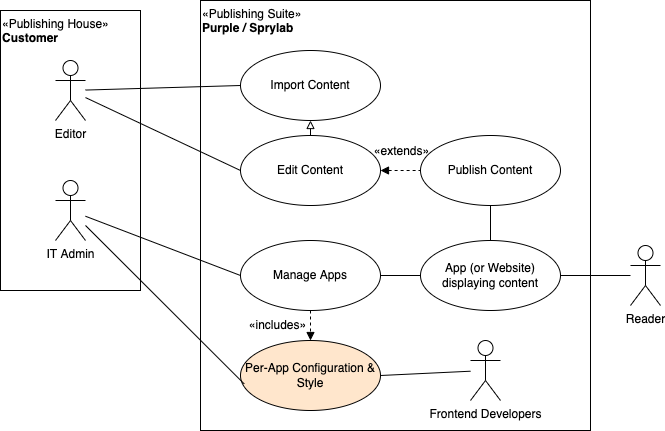
\includegraphics[width=\textwidth]{pics/purple-abstract.drawio.png}
  \label{fig:usecase1}
\end{figure}

The UI editor fits into the Use case ''Per App configuration \& style'' (see fig. \ref*{fig:usecase1}), with wich mostly Frontend Developers and Project Managers from Sprylab as well as some external customer's IT admins will interact. The goal is to lower the editing burden as much as possible, so that more of the configuration can be handed off to external customers while also improving usability for the developers of the company.

\subsection{Technical}
Now that we have established a rough understanding of the environment and use case the UI editor will be placed in, I want to explain more about the configuration and styling itself.
For that, it is important to understand the Frontend framework Sprylab uses for the delivery to apps and websites. It is called Purple Experience and is a Meta framework build ontop of Angular. The benefit is, that it is completely configurable via JSON files describing the routing, rendering of diffrent components,
connecting data sources (an API abstraction) with those components, loading assets like images and ads, and styling the whole page with CSS.
\\
These configs and assets are stored on an file system called \label{def:DynamicResources} \textit{dynamic resources}.
\\\\
Dynamic resources are individually managed and loaded for every app. This way, on mobile phones the endusers download an native core app, which in turn just downloads the dynamic resources and executes the angular app with the configs provided from the resources.
Similar, when a end user requests a website, the backend server just looks up the dynamic resources matching this app's Domain and renders the website using that config.
This way, all customers can share the same server instance(s) in case of websites, or at least don't require extra native sourcecode changes per app.
\\
In addition, there are preview and live resources for every app, so that changes can be tested before they are released to the end users.
\begin{figure}[h]
  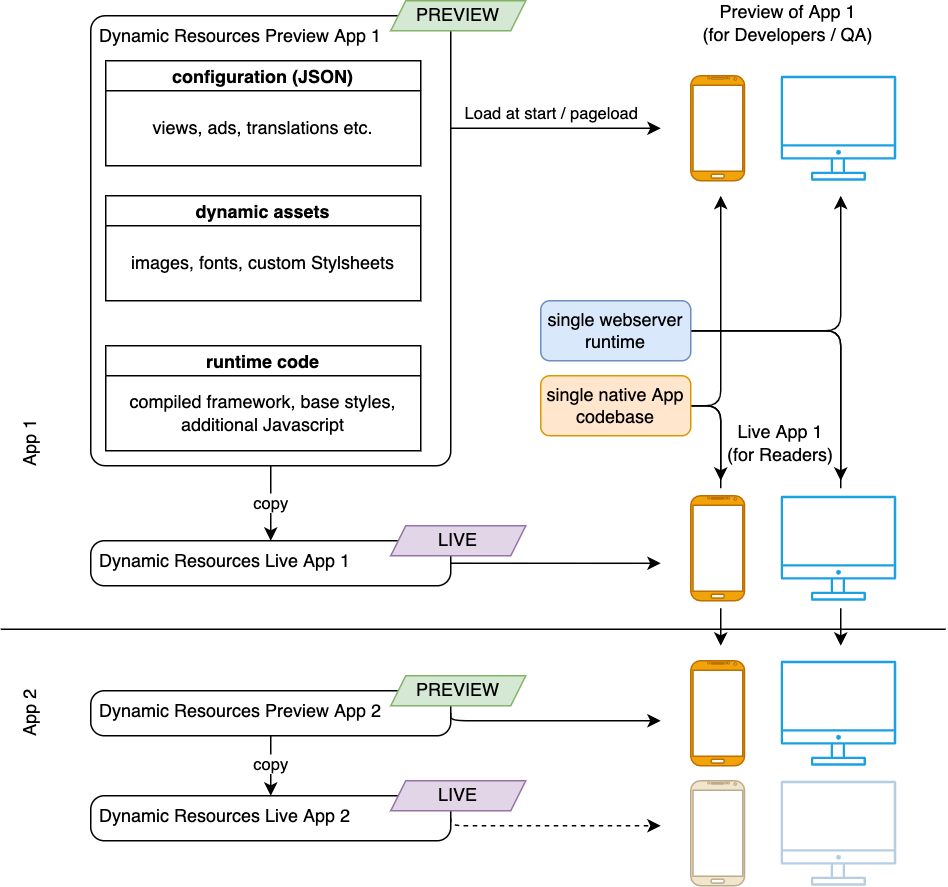
\includegraphics[width=\linewidth]{pics/experience_resources.drawio.png}
  \caption{Sprylab preview and live dynamic resources for two imaginary apps 1 and 2}
  \label{fig:dynres}
\end{figure}
\\
If you have worked with larger, deeply nested JSON files before, you may recall that they get convoluted quite fast.
Also, manually handling ZIP files, changing assets and config files, packing everything back in a zip file and hoping one didn't introduce a typo anywhere is an inefficient an at times quite dangerous workflow.
\\
As a base for making editing of these configuration JSON files easier, the Purple Experience generates JSON schema files directly from the Interfaces in the source code for every released version.
JSON Schema is a specification and a declarative language ''that allows you to annotate and validate JSON documents.'' (Retrieved 11th January 2023, from \url{https://json-schema.org/}).
With these schemas, it's possible to validate the users input directly and even generate UI Elements so that is impossible for the user to enter invalid JSON or JSON that doesn't match the
types declared in the source code.

At Sprylab, there exists an tool called ''Storefront Editor'', which is used as the foundation for this new editor.
It uses a open source software called \textit{Json Editor} (\url{https://github.com/json-editor/json-editor}), which takes a JSON schema and a matching JSON config as input and generates such a mentioned UI to manipulate the JSON in a safe way.
As part of the chapter \ref{chap:research} about User Research and Analysis, I evaluate the state of the JSON editor for that usecase and in general outline the positive aspects and approaches which I reused for the new editor,
as well show the missing features and features the interview candidates noted as confusing, not working or which slowed down their work.

\begin{figure}
  \lstset{language=json,basicstyle=\footnotesize,numbers=left,showstringspaces=false,frame=single}
  \begin{lstlisting}
{
  "type": "view",
  "path": "/newsstand",
  "content": [
    {
      "type": "list",
      "content": {
        "type": "issue"
      },
      "dataSource": {
        "type": "issue",
        "filter": {
          "purchasable": {
            "value": true
          }
        }
      }
    }
  ]
}
  \end{lstlisting}
  \caption{Simplified example of an view configuration showing purchasable issues}
\end{figure}